%\documentclass[twocolumn,amsmath,amssymb]{report}
\documentclass[twocolumn,amsmath,amssymb]{snp}
\pagestyle{empty}

\usepackage{graphicx}% Include figure files
\usepackage{dcolumn}% Align table columns on decimal point
\usepackage{bm}% bold math
\topmargin 1.5 cm
\textwidth14.5cm
\textheight20cm
\oddsidemargin0.7cm
\columnsep0.2in



\title{{\Large \LaTeX\ template and guidelines for preparing the contributory papers}}% Force line breaks with \\

\author{\large A. Author$^1$}
\email{aauthor@barc.gov.in}
\author{\large B. Author$^2$}
\author{\large C. Author$^3$}
\author{\large D. Author$^4$}%\email{abc@barc.gov.in}
% \altaffiliation[Also at ]{Physics Department, XYZ University.}%Lines break automatically or can be forced with \\
\affiliation{$^1$Nuclear Physics Division, Bhabha Atomic Research Centre, Mumbai - 400085, INDIA}
\affiliation{$^2$Deptartment of Nuclear and Atomic Physics, 
Tata Institute of Fundamental Research, Mumbai - 400005, INDIA}
\affiliation{$^3$Inter University Accelerator Centre, Aruna Asaf Ali Marg, New Delhi - 110067, INDIA}
\affiliation{$^4$Physics Department, XYZ University}



\maketitle


\section*{Introduction}
DAE Symposia on Nuclear Physics covering a wide range of topics \cite{poster} are conducted annually. The aim of this series of symposia has been to provide a scientific forum to the nuclear physics community to present their research work and to interact with the researchers in this area. 

{\bf This is a \LaTeX\ template for submission of poster contributions and thesis presentations}. 
An equivalent MS Word (*.doc file) version of this template 
is also available in the website.  
The bound volume of the 
symposium proceedings \cite{dae} will be distributed during the symposium. The two-page contributions, strictly in 
the form of this template, should be submitted in the website before the deadline.  Only the pdf version of the paper should be uploaded in the website. No hardcopy or email submission is acceptable. While submitting the paper, please mention the category of the topic 
under which your paper belongs.


\section*{Format of the Template}
The \LaTeX\ format which has been chosen here is very similar to that of Physical Review C format. Very few changes 
have been made in this format, e.g., in the sizes of the titles, authors, headings, textwidth, textheight, etc.
The sizes of the `title' and the `authors' are made larger using the command \verb+\Large{Title}+ and \verb+\large{author}+ respectively.
%The headings for the sections, subsections and sub-subsections are written using the commands \verb+\large{\bf Heading}+, \verb+{\bf subsection}+ and \verb+{\it subsubsection}+ respectively. 


\section*{Figures and Tables}
As the proceedings print will be in monocolor, all necessary figures, plots, spectra etc. have to be in 
black and white or grayscale with a good contrast so that good reproduction can be obtained. 
Following are the two ways to incorporate images into your LaTeX document.\\
%\begin{enumerate}
1. Include only PDF, PNG and JPEG images and use pdflatex, TeXShop, or other PDF-oriented compiler. The compiler pdflatex (unix/ winshell)  and TeXShop (Macintosh) convert LaTeX source directly to PDF, and do not accept PostScript images. Instead, they take PDF images, as well as bitmap pictures in PNG or JPEG format. So to use pdflatex, you must convert any PostScript images to one of these other forms. For photos, JPEG is best. For other bitmap images, PNG is best. For non-bitmap
images (e.g., graphs, drawings, stuff with text and symbols) it is best to convert to PDF, using the command epstopdf (in the usual TeX bin directory, e.g., /usr/local/tex/bin/epstopdf). With PNG or JPEG you should specify an explicit width or height rather than ``scale".\\
2. Include only PostScript images (esp. ``Encapsulated PostScript'') if your
goal is a PostScript document using dvips. Then you must compile the document with latex followed by dvips -Ppdf, which
produces a PostScript document with embedded PostScript images. You can convert
the PostScript document to PDF using ``ps2pdf'' or ``dvipdf''.
%\end{enumerate}

Fig.~\ref{fig1} shows a figure that is small enough to
fit in a single column. It is embedded using the \texttt{figure}
environment which provides both the caption and the imports of the figure
file.
\begin{figure}
\includegraphics[scale=1.5]{fig_1.eps}% Here is how to import EPS figure if you are using latex command to compile
%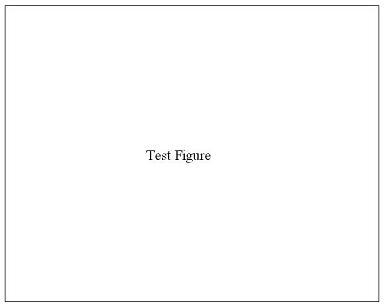
\includegraphics[width=66mm]{fig_1.jpg}% Here is how to import jpg/ png/ pdf figure if you are using pdflatex command to compile
\caption{\label{fig1} A figure caption. The figure captions are
automatically numbered.}
\end{figure}

\begin{table}[h]
\caption{\label{tab:table1}This is a table which fits
properly in a column. Note that several entries share the same
footnote. Inspect the \LaTeX\ input for this table to see
exactly how it is done.}
\begin{tabular}{|c|c|c|c|c|c|c|}
\hline 
&$r_c$ (\AA)& $r_0$ (\AA)& $\kappa r_0$&
 &$r_c$ (\AA) &$r_0$ (\AA)\\ \hline
Cu& 0.800 & 14.10 & 2.550 &Sn\footnotemark[1]
& 0.680 & 1.870 \\
Ag& 0.990 & 15.90 & 2.710 &Pb\footnotemark[2]
& 0.450 & 1.930  \\
Au& 1.150 & 15.90 & 2.710 &Ca\footnotemark[3]
& 0.750 & 2.120 \\
Mg& 0.490 & 17.60 & 3.200 &Sr\footnotemark[4]
& 0.900 & 2.370 \\
Zn& 0.300 & 15.20 & 2.970 &Li\footnotemark[2]
& 0.380 & 1.730 \\
\hline
\end{tabular}
\footnotetext[1]{Here's the first.}
\footnotetext[2]{Here's the second.}
\footnotetext[3]{Here's the third.}
\footnotetext[4]{Here's the fourth.}
\end{table}



The size of the figures and tables should not exceed the column width else it can be in two column width. When the figure is too wide for a single column, then use the \texttt{figure*} environment instead. Similarly for wide table one has to use 
\texttt{table*} environment.



\section*{Math and Equations}

Below we have numbered single-line equations; these are the most common
type of equations in \textit{Physical Review}:
\begin{equation}
\sigma = \pi R^2.  
\end{equation}
\begin{eqnarray}
\chi_+\alt{\bf [}2|{\bf p}|(p_z){\bf ]}^{-1/2}
\left(
\begin{array}{c}
|{\bf p}|+p_z\\
px+ip_y
\end{array}\right)\;.
\end{eqnarray}
\begin{eqnarray}
\left\{%
 \openone290ab13\alpha\beta\gamma\delta1256\alpha\beta
 \frac{1\sum^{a}_{b}}{A^2}%
\right\}%
\label{eq:one}.
\end{eqnarray}
Note the open one in Eq.~(\ref{eq:one}).

Unnumbered single-line equations can be typeset
using the \verb+\[+, \verb+\]+ format:
%\[g^+g^+ \rightarrow g^+g^+ \dots ~,~~q^+q^+\rightarrow
%q^+g^+ \dots ~. \] 
\[n+p \rightarrow d+\gamma ~,~~n+d\rightarrow
t+\gamma ~. \] 



\section*{General Guidelines}
Once the paper is written as per the format either in MS Word or in \LaTeX\, it should be converted to a pdf file. 
In the authors' list, in 
case of a large collaborative experiment it is advised to mention the name of the collaboration and spokesperson's 
email address instead of the complete list of authors. For references also, the name of collaboration or only the 
``first author, et al.'' style can be adopted. 

It is not encouraged to have the figures and tables together to occupy more than 50\% of available area. Also the content should be sufficient and complete. Authors are also expected not to split their work to submit multiple contributions.

Although the contributions are in soft copy form, the symposium organizer will not make any attempt to 
edit it to conform to the template format.  After screening of the contributions, the 
acceptance status of the papers shall be made available only on the website 


\section*{Acknowledgments}
%\acknowledgments
 We thank you for your co-operation in using this template  for production of camera ready manuscript.
%\end{acknowledgments}

%\ \\
%\noindent
\begin{thebibliography}{50}
\bibitem{poster} Announcement Poster and Website, DAE Symp. {\bf vv}, ppp (yyyy).
\bibitem{dae} DAE Symp. on Nucl. Phys. {\bf vv}, ppp (yyyy).
\end{thebibliography}

\end{document}
%
% ****** End of file snpcontrisamp.tex ******
